\documentclass{article}

\usepackage{graphicx}
\usepackage{tikz}
\usepackage{tikzsymbols}
\usetikzlibrary{calc,patterns,shapes.geometric}
\pagestyle{empty}
\usepackage[margin=0pt]{geometry}
\geometry{papersize={14in,12in}}

\def\centerarc[#1](#2)(#3:#4:#5){\draw[#1] ($(#2)+({#5*cos(#3)},{#5*sin(#3)})$) arc (#3:#4:#5);}

\begin{document}
	\begin{figure}
		\centering
		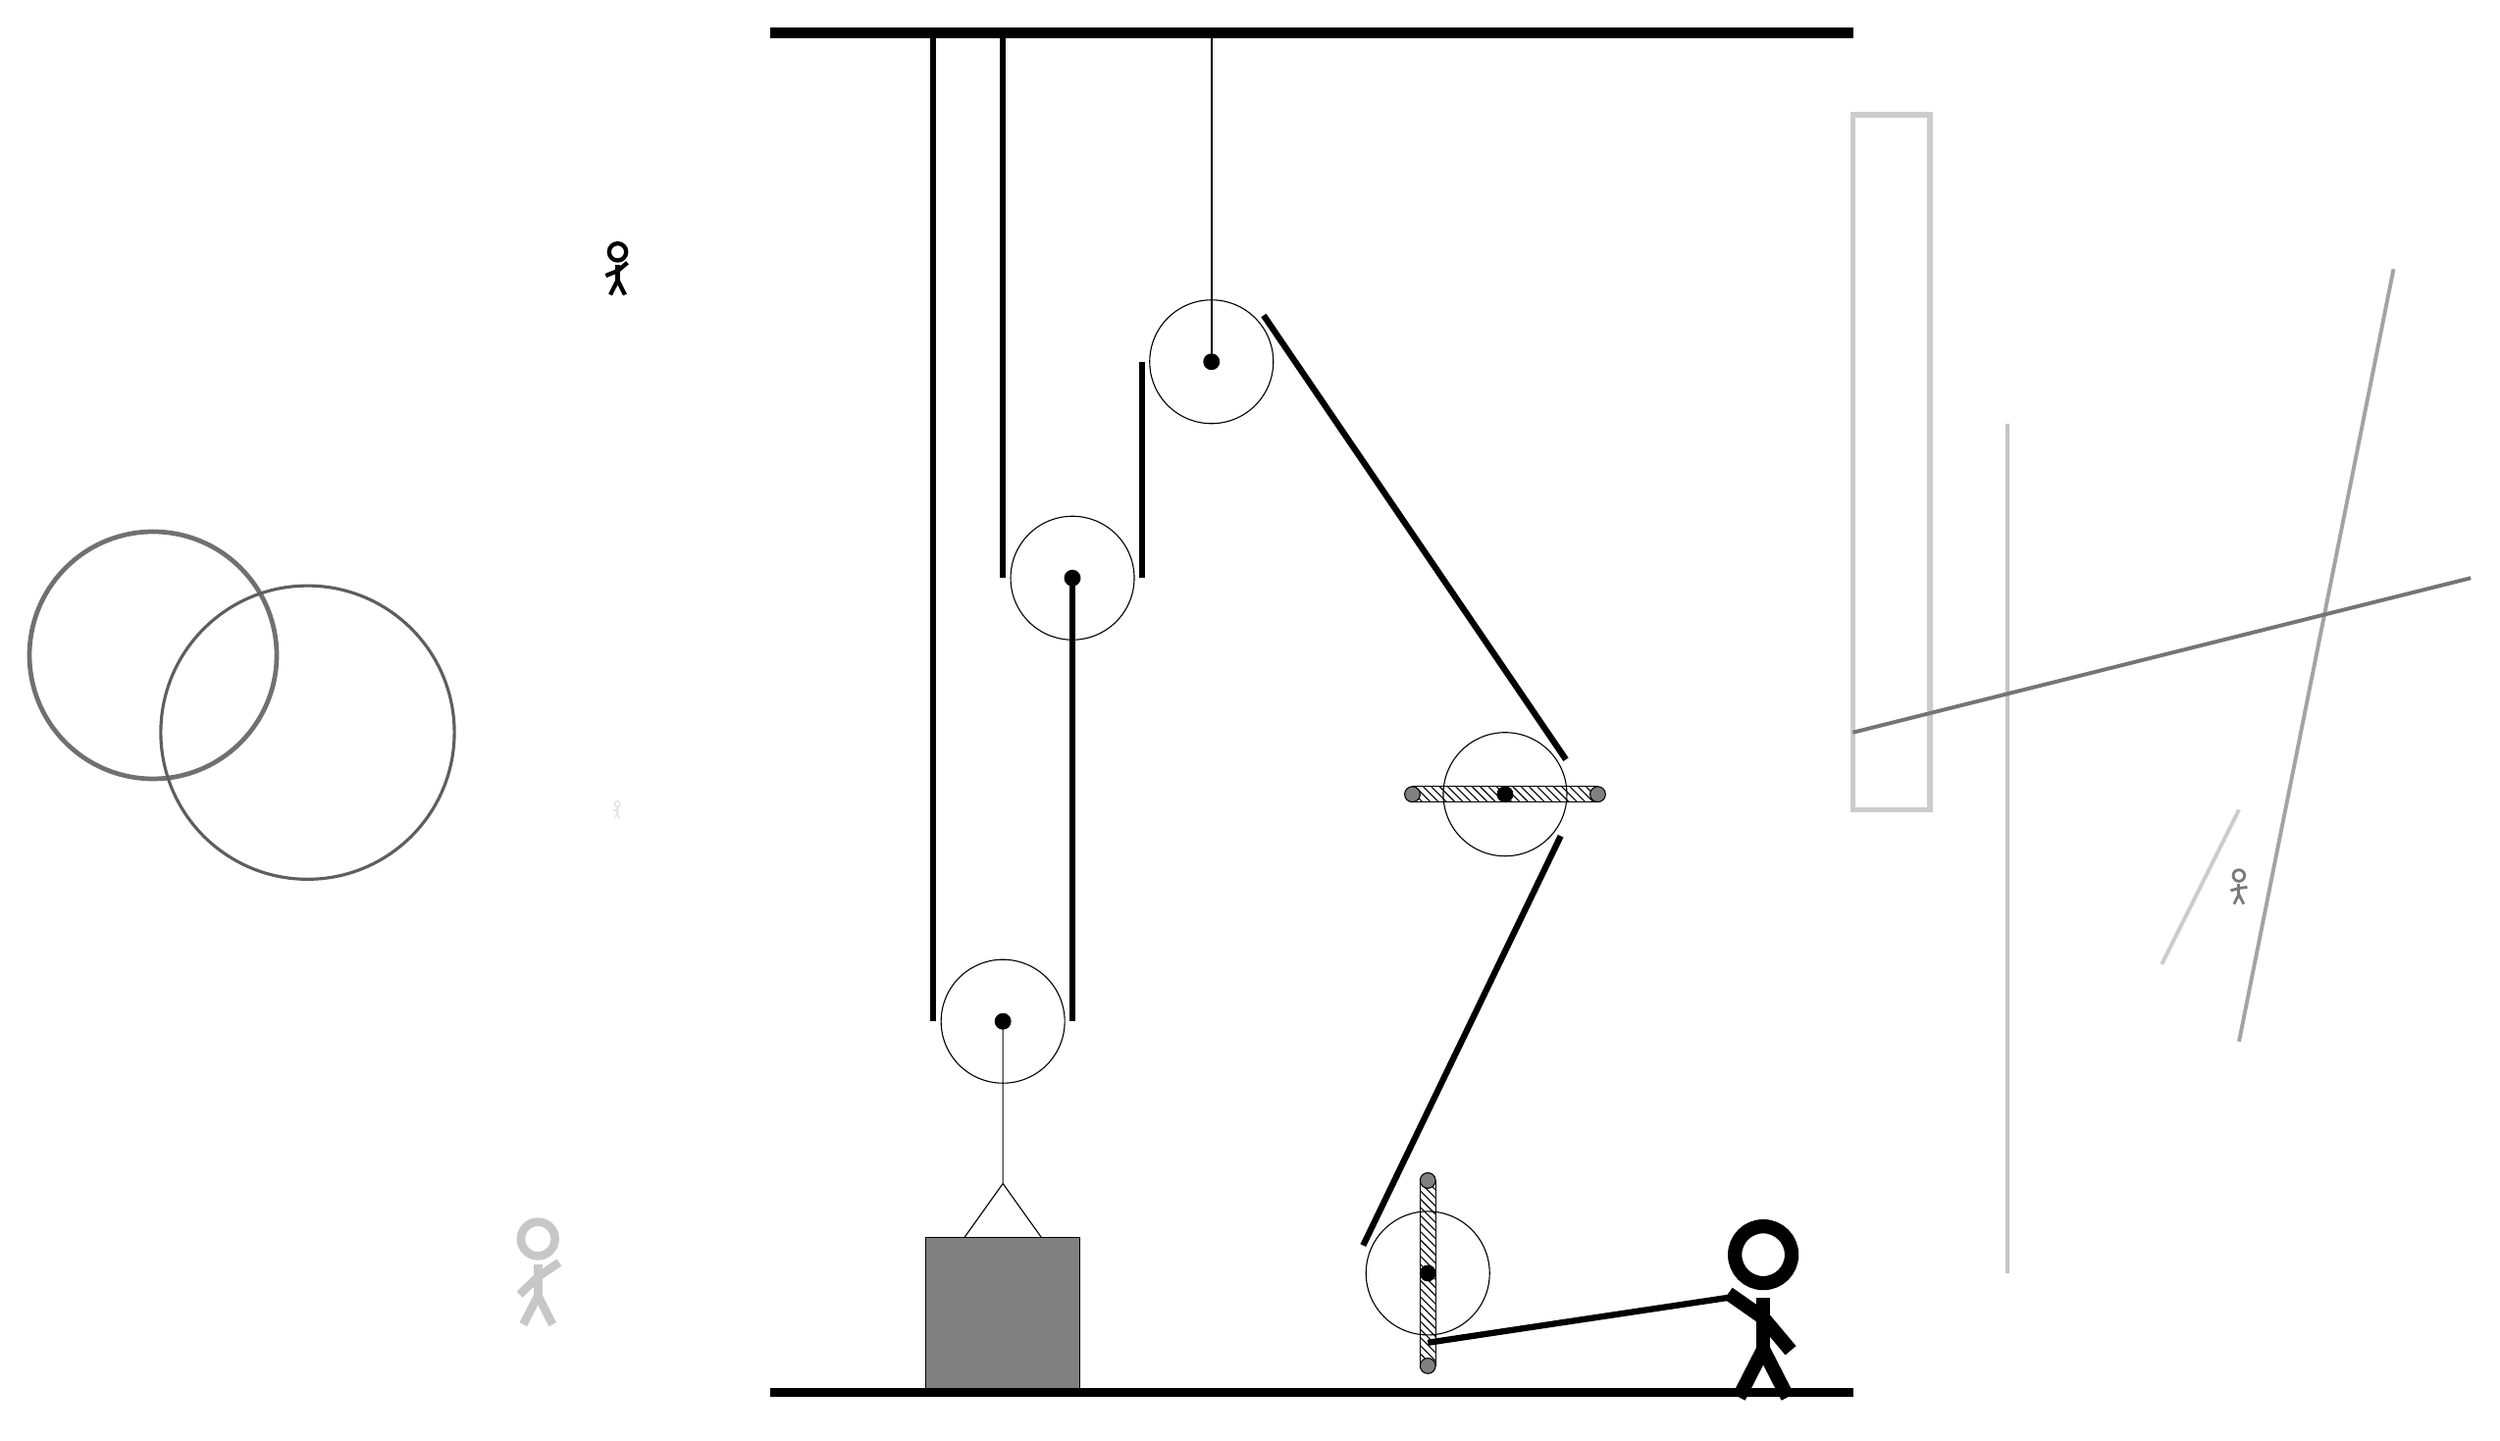
\begin{tikzpicture}
			%%%%% START %%%%%
			
			\draw[fill=black] (-2, 14) rectangle (12, 14.125);
			
			\draw (1, 1.26) circle (0.8);
			\draw[fill=black] (1, 1.26) circle (0.1);
			
			\draw (1.9, 7.0) circle (0.8);
			\draw[fill=black] (1.9, 7.0) circle (0.1);
			
			\draw (3.7, 9.8) circle (0.8);
			\draw[fill=black] (3.7, 9.8) circle (0.1);
			\draw[thick] (3.7, 9.8) -- (3.7, 14);
			
			\draw (6.5, -2) circle (0.8);
			\draw[fill=black] (6.5, -2) circle (0.1);
			\draw[pattern=north west lines, pattern color=black] (6.4, -0.8) rectangle (6.6, -3.2);
			\draw[fill=black!50] (6.5, -0.8) circle (0.1);
			\draw[fill=black!50] (6.5, -3.2) circle (0.1);
			
			\draw (7.5, 4.2) circle (0.8);
			\draw[fill=black] (7.5, 4.2) circle (0.1);
			\draw[pattern=north west lines, pattern color=black] (6.3, 4.3) rectangle (8.7, 4.1);
			\draw[fill=black!50] (6.3, 4.2) circle (0.1);
			\draw[fill=black!50] (8.7, 4.2) circle (0.1);
			
			\draw (1, 1.26) -- (1, -0.84) -- (0.5, -1.54) -- (1.5, -1.54) -- (1, -0.84);
			\draw[fill=black!50] (0, -1.54) rectangle (2, -3.54);
			
			\draw[line width=0.8mm] (0.1, 14) -- (0.1, 1.26);
			\centerarc[line width=0.8mm](1, 1.26)(180:360:0.9);
			\draw[line width=0.8mm](1.9, 1.26) -- (1.9, 7.0);
			\draw[line width=0.8mm] (1.0, 14) -- (1.0, 7.0);
			\centerarc[line width=0.8mm](1.9, 7.0)(180:360:0.9);
			\draw[line width=0.8mm](2.8, 7.0) -- (2.8, 9.8);
			\centerarc[line width=0.8mm](3.7, 9.8)(35:180:0.9);
			\draw[line width=0.8mm] (4.375, 10.4) -- (8.2875, 4.65);
			\centerarc[line width=0.8mm](7.5, 4.2)(215:135:-0.9);
			\draw[line width=0.8mm](8.22, 3.66) -- (5.663, -1.64);
			\centerarc[line width=0.8mm](6.5, -2)(-30:100:-0.9);
			\draw[line width=0.8mm](6.5, -2.9) -- (10.5, -2.3);
			
			\node[line width=0.3mm, color=black!52] at (17, 3) {\Strichmaxerl[2][16][7]};
			
			\draw[line width=0.7mm, color=black!20] (12, 4) rectangle (13, 13);
			\node[line width=0.3mm, color=black!22] at (-5, -2) {\Strichmaxerl[6][44][34]};
			\node[line width=0.7mm, color=black!100] at (-4, 11) {\Strichmaxerl[3][22][40]};
			\draw [line width=0.6mm, color=black!56](-10, 6) circle (1.6);
			\draw[line width=0.5mm, color=black!20](17, 4) -- (16, 2);
			
			\node[line width=0.5mm, color=black!11] at (-4, 4) {\Strichmaxerl[1][0][73]};
			\draw[line width=0.5mm, color=black!23](14, -2) -- (14, 9);
			\draw [line width=0.4mm, color=black!63](-8, 5) circle (1.9);
			\draw[line width=0.5mm, color=black!36](17, 1) -- (19, 11);
			\draw[line width=0.5mm, color=black!54](12, 5) -- (20, 7);
			
			
			\node at (10.8, -2.5) {\Strichmaxerl[10][-35][-50]};
			
			\draw[fill=black] (-2, -3.5) rectangle (12, -3.6);
			
			%%%%% END %%%%%
		\end{tikzpicture}
	\end{figure}	
\end{document}